\capitulo{5}{Aspectos relevantes del desarrollo del proyecto}

En este apartado se van a recoger los aspectos más importantes del desarrollo
del proyecto. Desde las decisiones que se tomaron y sus implicaciones,
hasta los numerosos problemas a los que hubo que enfrentarse y cómo se
solucionaron.

\section{Elección del proyecto}

A finales del curso pasado se organizó una charla en la que los profesores iban
a presentar las optativas que daban clase de forma que los alumnos tuviéramos
más fácil elegir asignaturas. En la presentación de la asignatura ``Minería de
Datos'' despertó interés por el tema y se preguntó a José Francisco, por haber
realizado la presentación, sobre TFGs relacionados con el tema.

De los trabajos disponibles este llamó la atención por estar relacionados con
geología y con desarrollo web, además de poder aplicar técnicas minería de datos
en un entorno real de investigación.

\section{Formación}

Para poder realizar el proyecto se necesitaban unos conocimientos no adquiridos
sobre desarrollo web, tanto de la parte de servidor en Flask como la parte del
cliente en HTML, CSS y JavaScript, aunque en menor medida por haberse tocado
algo durante el grado. Como se había hablado con los tutores antes de verano
sobre el proyecto, se dedicó parte a aprender sobre ello. Además de para
aprendizaje, los recursos se han usado también como material de consulta durante
el desarrollo.

\noindent Para la parte del servidor se siguieron los libros y tutoriales:
\begin{itemize}
	\item Flask Web Development\cite{grinberg2014flask}
	\item Explore Flask\cite{exploreflask}
	\item The Flask Mega-Tutorial Legacy (2012)\cite{grinberg-mega-legacy}
	\item The Flask Mega-Tutorial (2017)\cite{grinberg-mega}
\end{itemize}

\noindent Para la parte del cliente se utilizaron principalmente los siguientes
materiales:
\begin{itemize}
	\item MDN Web Docs\cite{mdn}
	\item W3Schools Tutorials\cite{w3schools}
\end{itemize}

A medida que se añadían nuevas herramientas al proyecto, su documentación
oficial también ha sido consultada en varias ocasiones, están disponibles en:
\begin{itemize}
	\item Documentación de Flask\cite{doc:flask}
	\item Documentación de Bootstrap\cite{doc:bootstrap}
	\item Documentación de Nanobox\cite{doc:nanobox}
	\item Documentación de PyMongo\cite{doc:pymongo}
	\item Documentación de Dash\cite{doc:dash}
	\item Documentación de Plotly\cite{doc:plotly}
\end{itemize}

\section{Sistema de usuarios}

Uno de los primeros problemas que se plantearon fue la forma de ofrecer el
sistema de usuarios, para que cada uno pudiera almacenar sus archivos. Las
opciones que se presentaban eran implementar uno desde cero con ayuda de las
extensiones que ofrece Flask o mediante un sistema de terceros, como puede ser
Google.

Implementar el sistema desde cero tenía la ventaja de que los usuarios no tenían
que salir de la página para iniciar sesión y que se había aprendido como hacerlo
en los tutoriales sobre Flask mencionados anteriormente, mientras que el sistema
de terceros no se sabía como hacerlo, pero tenía más ventajas, siendo las
principales no tener que mantener una base de datos de usuarios, no depender de
un sistema de envío de correo electrónico (dio problemas en proyectos
anteriores) y no tener que obligar a los usuarios a crearse otra cuenta al poder
usar una existente.

Al final se decidió usar la autenticación con Google, por estar casi garantizado
que los usuarios van a tener una cuenta existente, la documentación sobre este
aspecto es abundante y era fácil de implementar. Además al iniciar sesión con
este servicio nos permite usar la API de Google para obtener los datos del
usuario necesarios.

\section{Cohesión entre Flask y Dash}

Al contar con la presencia de dos \textit{frameworks} de desarrollo web hacer
que funcionen juntos ha sido un reto, sobre todo teniendo en cuenta que Dash se
ejecuta Flask pero no permite reutilizar sus componentes, favoreciendo la
aparición de código repetido y disminuyendo la mantenibilidad.

El mayor problema que se ha tenido ha sido la diferencia en como escribir el
código HTML para la interfaz en el cliente. Mientras que en Flask se escribe en
ficheros HTML llamados \textit{templates}, Dash apuesta por escribir todo el
código desde Python. Esto favorece que surjan defectos de código, sobre todo de
código duplicado.

Se investigó bastante sobre cómo poder usar los \textit{templates} de Flask para
definir la interfaz de Dash pero no se pudo encontrar forma de poder hacerlo. Al
final no quedó otra forma de hacerlo, pero dentro de lo malo es un pequeño
precio a pagar por el resto de ventajas que Dash ofrece.

\section{Subida de ficheros}\label{sec:subida}

Una de las primeras características que se implementó fue la subida de ficheros
al servidor, al tener ya el sistema de usuarios se podían organizar los datos
sin problema para cada cliente. El formato requerido para subir los datos pasó
por varios cambios motivados por la forma en la que Susana nos enviaba los datos
que probar la aplicación. En secciones posteriores se explica como estos cambios
afectaron también al almacenamiento de los datos y la interfaz del visor.

\subsection{Organización en directorios}\label{sec:directorios}

Al principio los datos se encontraban organizados en directorios cuyo nombre
proporcionaba toda la información sobre los ejemplos que contenían. Por lo que
el formato que se pedía era simple, un archivo comprimido en formato ``.zip''
que contuviera estos directorios.

\subsection{Estructura según hoja de metadatos}\label{sec:excel}

Sobre mediados de Abril los nuevos datos recibidos empezaron a estar organizados
según una hoja de Excel que relacionaba los nombres de directorios y los
ejemplos que contenían con sus metadatos, en vez de estar contenidos en el
nombre.

Esta hoja contenía una columna llamada ``Id'' con el nombre de un directorio y
los ejemplos de ese tipo, las siguientes columnas contenían datos sobre los
ejemplos contenidos en esa fila, como la mina de la que han sido extraídas las
muestras o la profundidad.

Esta hoja se adaptó para aplicación manteniendo la columna ``Id'' y añadiendo
fijas una columna para la mina y otras dos para la profundidad, una nominal y
otra numérica. El formato de subida pasó a ser en un mismo fichero ``.zip'' los
directorios que contienen los ejemplos y la hoja con los metadatos previamente
cumplimentada.

\section{Interfaz del visor}

Esta parte del proyecto está muy relacionado con lo explicado en la
sección~\ref{sec:subida}, el usuario del visor espera que se le presenten los
datos de una forma similar a como los ha subido.

Cuando los datos se subían como un archivo comprimido con carpetas cuyo nombre
contiene la información se presentaban al usuario dos menús desplegables. En la
carga solo uno de ellos contenía valores, los nombres de los directorios. El
segundo desplegable actualizaba sus valores con los nombres de los ficheros
contenidos en la carpeta seleccionada, al seleccionar el fichero se cargaba en
el visor.

Con el cambio de la hoja con metadatos, el tutor José Francisco propuso que al
usuario se le mostrase una tabla parecida al hoja que había rellenado antes de
subir los datos, con la diferencia de que se mostrasen todos los ficheros como
filas con sus metadatos, asemejándose a la estructura final de almacenamiento de
datos.

Mostrar los datos al usuario en forma de tabla trajo las ventajas de poder
representar varios espectros a la vez, filtrar y ordenar según las columnas (ver
Figura~\ref{fig:tabla-espectros}).

\imagen{tabla-espectros}{Tabla de espectros} 

\section{Almacenamiento de datos}

El principal motivo de implementar un sistema de usuarios fue que cada uno
pudiera tener sus datos almacenados para no tener que subirlos cada vez que se
quiera trabajar con ellos.

\subsection{Inicialmente}

Al principio se almacenaban directamente en un directorio nombrado como el id
del usuario y lo único que se hacía era descomprimir el archivo comprimido en
ese directorio. Esta forma de almacenar los datos conlleva varios problemas que
motivaron el cambio en la forma de almacenamiento a la actual. Esta forma de
almacenamiento se corresponde al formato explicado en la
sección~\ref{sec:directorios} (Organización en directorios).

El problema más evidente, y que más notarían los usuarios, es que cada vez que
se quisiera ver un espectro hay que cargarlo desde el disco, disminuyendo el
rendimiento general de la aplicación.

Otro gran problema de esta forma de almacenar era como manejaba el servidor los
ficheros guardados, este tema se explicará más en detalle en la
sección~\ref{sec:despliegue}.

El último problema y el más problemático desde el punto de vista de programación
es que para cada operación que se quisiera realizar con los datos se necesitaban
escribir funciones auxiliares complejas para buscar y manipular el árbol de
directorios, las cuáles había que modificar con cada cambio en la estructura,
dificultando el mantenimiento de la aplicación.

Se planteó cambiar la forma de almacenar los datos en el servidor, cambio que
terminó por realizarse después de valorar ventajas y desventajas en este momento
del desarrollo.

\subsection{Migración a MongoDB}

Por sugerencia del tutor se investigó la posibilidad de usar MongoDB para
almacenar los datos. Se vio que podría funcionar realmente bien al poder
insertar directamente los ficheros cargados en la base de datos, recuperarlos y
borrarlos fácilmente. Como consecuencia directa del cambio los métodos
auxiliares con los que se interactuaba con los datos disminuyeron
considerablemente en tamaño y complejidad.

En primera instancia se optó por guardar los conjuntos de datos como un
documento en el que estaban contenidos varios \textit{DataFrames} (cada uno
representando un espectro) agrupados según la carpeta en la que estuvieran
localizados los espectros. Cada \textit{DataFrame} contenía dos columnas, una
con los valores del eje X y otra con los valores del eje Y.

Pero seguido de adoptar esta estructura y tener la aplicación adaptada para ello
llegó el cambio en como recibíamos los datos, provocando otra modificación en la
estructura. Esta vez se decidió agrupar todo el conjunto de datos subido en un
solo \textit{DataFrame}, en el que cada fila se corresponde con un espectro, las
columnas representan el eje X y los valores de cada fila en esas columnas
representan el valor del eje Y. Cada fila contiene adicionalmente columnas que
indican el nombre del espectro y sus metadatos asociados (ver
Figura~\ref{fig:dataframe-def}). En la sección~\ref{sec:integracion} se explican
más en profundidad este cambio.

\begin{figure}[!h]
	\centering
	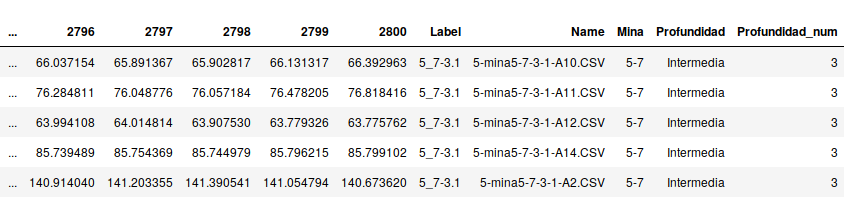
\includegraphics[width=\textwidth]{dataframe-def}
	\caption{Estructura definitiva}\label{fig:dataframe-def}
\end{figure}

Guardar los datos de esta forma facilita aplicar los métodos de minería de datos
al estar pensado para aplicarse en lote.


\section{Integración de los algoritmos existentes}\label{sec:integracion}

Como se ha comentado en la introducción (página~\pageref{ch:introduccion}), este
proyecto surge de una colaboración. De aquí se obtuvieron bastantes algoritmos,
gran parte de ellos dedicados al procesamiento de los espectros, que se
añadieron sobre la librería ``superman'' (\ref{lib:superman}).

Una de las partes más importantes del proyecto era conseguir integrar estos
algoritmos en la aplicación web para poder ejecutarlos sobre los espectros
visualizados.

Cuando llegó el momento de integrarlos algoritmos en la aplicación había dos
opciones para hacerlo funcionar, modificar la aplicación para adaptarse a los
algoritmos o modificar los algoritmos para adaptarse a la aplicación.

En primera instancia se intento modificar los algoritmos pero se vio que era un
paquete con demasiadas dependencias dentro del propio paquete, por lo que cada
cambio producía gran cantidad de errores de funcionamiento, que al solucionar
producían todavía más errores dentro del paquete. Se optó por revertir estos
cambios y modificar la aplicación.

La modificación principal fue la modificación final en como guardar los datos
comentada anteriormente (figura~\ref{fig:dataframe-def}). Con esa modificación
el funcionamiento de la aplicación volvió a ser el correcto.

\section{Despliegue}\label{sec:despliegue}

La idea de realizar el proyecto como una aplicación web tiene relación más que
directa con que pueda estar accesible en pocos clicks. Para ello se necesita que
esté desplegada y accesible en Internet. En esta sección de describe las etapas
por las que pasó el despliegue, los problemas que surgieron y como se
solucionaron.

En las primeras reuniones del proyecto se comentó con los tutores que un gran
problema de los proyectos anteriores desarrollados en web se centraban en el
despliegue al final del proyecto, haciendo que alguna vez no pudieran llegarse a
desplegar, por eso se planteó la idea de empezar a desplegar desde el inicio del
proyecto.

\subsection{Servidor}

La plataforma escogida fue
\href{https://www.heroku.com/}{Heroku}\footnote{\url{https://www.heroku.com/}}
por su simplicidad y un plan gratuito que cubre las necesidades del proyecto.
Aunque en primera instancia parecía que esta plataforma funcionaba bien para
nuestras necesidades se vio que no contaba con almacenamiento persistencia,
convirtiendo su uso en inviable.

Las opciones que se plantearon fueron buscar una forma de añadir este
almacenamiento y cambiar de servidor por completo. Para añadirlo en Heroku había
que depender de \textit{plugins} de terceros para enlazar servicios de
almacenamiento de terceros teniendo que modificar la aplicación para hacerlo
funcionar, además de ser servicios de pago.

Al final se escogió por cambiar a un proveedor \textit{cloud} de pago que
ofreciese máquinas virtuales privadas, las opciones manejadas fueron
\href{https://www.digitalocean.com/}{DigitalOcean}\footnote{\url{https://www.digitalocean.com/}},
\href{https://aws.amazon.com/es/}{Amazon Web
	Services}\footnote{\url{https://aws.amazon.com/es/}} y
\href{https://cloud.google.com/}{Google
	Cloud}\footnote{\url{https://cloud.google.com/}}. Se escogió la primera opción
ya que gracias al \href{https://education.github.com/pack}{Student Developer
	Pack}\footnote{\url{https://education.github.com/pack}} se disponía de un cupón
de 50\$ en esta plataforma.

\subsection{Herramientas para el despliegue}

La plataforma Heroku posee sus propias herramientas para el despliegue,
facilitando en gran cantidad este proceso. Esta plataforma un repositorio
\textit{git} remoto para almacenar la aplicación por lo que al contar ya con
este sistema de control de versiones en el proyecto no hubo que modificar casi
nada para poder desplegar, pero por lo problemas comentados anteriormente se
tuvo que abandonar.

Para complementar a DigitalOcean y facilitar la tarea del despliegue se ha usado
el servicio
\href{https://nanobox.io/}{Nanobox}\footnote{\url{https://nanobox.io/}}. Al
principio de usar esta plataforma se vio que los datos almacenados se eliminaban
en cada despliegue, para ello hubo que añadir un segundo contenedor que se
ocupara del almacenamiento, lo bueno es que este contenedor se asocia a un
directorio del servidor, por lo que la aplicación no se tuvo que modificar. Más
adelante se añadió otro contenedor para gestionar la base de datos MongoDB.

\section{Creación de clasificadores}

Dentro del objetivo de aplicación de técnicas de minería de datos había que
decidir si dejar a los usuarios la opción de crear clasificadores personalizados
o simplemente entrenarlos a partir de \textit{datasets} subidos. Se decidió
probar la primera opción, teniendo la segunda como respaldo en caso de no
funcionar.

\subsection{Obtención de parámetros}

Para conseguir esta personalización surge el problema de cómo obtener los
parámetros del clasificador y presentárselos al usuario. La primera idea que
surgió es analizar la documentación oficial de los clasificadores y crear a mano
un fichero con los parámetros, esto puede resultar viable si se usan pocos
clasificadores pero dificulta mucho la adición de nuevos.

Se descartó a favor de buscar una herramienta que pudiera analizar la
documentación \textit{in-code} de los clasificadores. Al ser un formato
estructurado y conociendo herramientas en otros lenguajes de análisis de este
tipo de documentación seguro que para Python existen herramientas parecidas.

Se encontró la librería
\href{https://github.com/numpy/numpydoc}{numpydoc}\footnote{\url{https://github.com/numpy/numpydoc}}
que, entre otras características, ofrece la funcionalidad que se busca, analiza
la documentación y devuelve un diccionario con las secciones, entre ellas los
parámetros.

Con esta información se puede generar un formulario automáticamente y hacer que
cambie dinámicamente según la opción del usuario.

\subsection{Procesamiento del formulario}

El servidor recibe todos los datos como si fueran cadenas, aunque el control en
el formulario sea de tipo numérico, por lo toca convertir las cadenas al tipo
correcto con un método de prueba y error, para luego guardarlos y pasárselos al
constructor del clasificador. Si no se ha introducido valor no se guarda
permitiendo usar el valor por defecto.

Primero si el valor coincide con un \textit{booleano} se convierte, si no se
prueba a convertir en entero, si salta excepción se prueba a convertir en
numérico con decimales, en caso de que salte excepción, al no haber más tipos
primitivos se asume que el valor tiene que ser una cadena y guarda como tal.

\subsection{Mantener el modelo entre peticiones}

Al ser los clasificadores creados y personalizados desde la web, estos
necesariamente se tienen que crear mientras se procesa la petición, con su
consecuente destrucción al terminar de procesarla, con lo que la tarea de
guardarlos se complica.

Las ideas propuestas para solventar el problema fueron guardar los parámetros
usados como una \textit{cookie} para poder entrenar el modelo otra vez antes de
guardarlo o serializar el modelo ya entrenado en el servidor temporalmente y
cargarlo en caso de querer guardarlo definitivamente.

A pesar de la facilidad de usar \textit{cookies} para solucionar el problema,
estos datos guardados son necesarios solo en el caso de que se elija guarda el
modelo, por lo que parece algo precipitado guardarlos cuando puede que no se
lleguen a usar.

Sin embargo la razón para descartar esta idea es la confianza que se ofrece al
usuario. Si se reentrena el modelo, aunque sea con los mismos parámetros, la
separación que se hace de los datos en entrenamiento y test puede ser diferente,
resultando en un clasificador diferente con estadísticas diferentes.

La opción de serialización permite centralizar todo en el servidor, permitiendo
una fácil carga y guardado del modelo entrenado, solucionando el problema de la
confianza. Además se evita el envío de datos innecesarios al usuario en cada
petición. Por último, el servidor está configurado para vaciar el almacenamiento
temporal cada día evitando el problema de almacenar datos que puede que no se
usen, porque la decisión de guardar el clasificador se toma justo después de
evaluarlo. 
